\section{Method}

Our work starts with a comprehensive overview of the underlying core concepts. As graph states lie at the heart of measurement-based quantum computing, it is necessary to introduce the terminology and some fundamental results. To make this introduction, we use two different approaches to define graph states. Next, we will introduce the one-way quantum computer, an abstract machine for quantum computing. We use this machine in the following section to discuss various results about measurement-based quantum computing.

\subsection{Graph States}

We start by introducing the necessary terminology regarding graphs, which are mathematical objects commonly used in computer science composed of vertices and edges. A graph is defined by a set \(V\) of \(N\) vertices and a set \(E\) of \(M\) edges\cite{clrs}.
\begin{gather}
  V = \Set{1, 2, \dots, N} \\
  E \subseteq [V]^2 \;\text{where}\; \abs{E\,} = M
\end{gather}
We usually represent graphs via diagrams. Such a diagram is given in Figure \ref{fig:graph_example}. As we do not impose order among the vertices that are connected by an edge, an edge is used only to denote \emph{connectivity}. Two vertices \(a, b \in V\) are called \emph{adjacent} if they are connected by an edge. The \emph{neighbourhood} of a vertex \(a \in V\) is the set of all the vertices \(a\) is adjacent to.
\begin{equation}
  N_a = \Set{\,b\in V \given \Set{a, b}\in E\,}
\end{equation}
Graphs that contain no loops---edges connecting a vertex to itself---or multiple edges between any two of its vertices are called \emph{simple graphs}\cite{hein2006}. The main type of graphs we deal with are simple graphs.

\begin{figure}[h]
  \centering
  \tikz \graph [
    ] {
      1 -- {2 -- 3, 4};
      3 -- 4;
    };
  \caption{The diagram of graph \(G = \{\Set{1,2,3,4}\,,\, \{\Set{1,2}, \Set{1,4}, \Set{2,3}, \) \(\Set{1,4}\}\} \) }\label{fig:graph_example}
\end{figure}

Simple graphs can be used to represent some interactions of qubit systems. We call these systems \emph{graph states}. Formally defining a graph state can be done in two different ways. The first one is by using the system's interaction patterns. 

A graph state described by the graph \(G = \Set{V, E}\) is made up of qubits that are labelled by the vertices of \(G\). Any two qubits \(a,b\in V\) connected by an edge \(\Set{a,b} \in E\) interact via an Ising type interaction. We also impose the following conditions apart from the restriction on the qubits' interaction type.
\begin{enumerate}
  \item Since an edge only denotes connectivity, all two-particle unitaries acting on a vertex must commute.
  \begin{equation}
    [U_{ab}, U_{bc}] = 0 \quad \forall a, b, c \in V
  \end{equation}
  \item Since edges do not denote a direction, unitaries must be symmetric.
  \begin{equation}
    [U_{ab}, U_{ba}] = 0 \quad \forall a, b \in V
  \end{equation}
  \item All the particles must interract through the same unitary.
\end{enumerate}
The general form of an Ising type interaction that satisfies these additional constraints is given by the following unitary, parameterized by the \emph{interaction strength}.
\begin{equation}
  U_{ab}^I(\psi_{ab}) = e^{-i \psi_{ab} \, \sigma_z^a \, \sigma_z^b}
\end{equation}
This interraction pattern is useful to us because of the entanglement patterns it produces. Note that such a unitary with parameter \(\psi_{ab} = \pi/4\) is equivalent to a controlled \(\sigma_z\) gate---denoted by CZ---up to some additional \(\pi/4\)-rotations around the \(z\) axis for each qubit.
\begin{equation}
\begin{aligned}
  e^{-i\frac{\pi}{4}} e^{i\sigma_z^a\frac{\pi}{4}} e^{i\sigma_z^b\frac{\pi}{4}} U^I_{ab}\p*{\frac{\pi}{4}} &= e^{-i\frac{\pi}{4}} e^{i\sigma_z^a\frac{\pi}{4}} e^{i\sigma_z^b\frac{\pi}{4}} e^{-i \frac{\pi}{4} \, \sigma_z^a \, \sigma_z^b}\\
  &= e^{-i\frac{\pi}{4}}\\
  &= \begin{bmatrix}
    1 & 0 & 0 & 0 \\
    0 & 1 & 0 & 0 \\
    0 & 0 & 1 & 0 \\
    0 & 0 & 0 & -1
  \end{bmatrix}
\end{aligned}
\end{equation}
Using CZ to construct edges makes sure that a resulting edege
\begin{equation}
  U_{ab}\ket+^a\ket+^b = \frac{1}{\sqrt2}(\ket0^a\ket+^b + \ket1^a\ket-^b) 
\end{equation}
is maximally entangled. Furhtermore \(U_{ab}\)\/ is Hermitian so it can be used to delete an edge as well.

A graph state \(\ket{G}\) which correspond to the simple graph \(G=\p{V, E}\) is defined to be
\begin{equation}
  \ket{G} = \prod_{\p{a,b} \, \in E} U_{ab}\,\ket+^V,
\end{equation}
and is prepared via the following procedure\cite{hein2006}.
\begin{enumerate}
  \item For each vertex in \(V\), prepare the corresponding qubit with the positive \(\sigma_x\) eigenstate \(\ket+\).
  \item For each edge \(\p{a,b}\in E\), apply \(U_{ab}\) to the system.
\end{enumerate}

\begin{figure}[bt]
  \centering
  \subcaptionbox{The diagram of \(G\)}[0.85\linewidth]{\begin{tikzpicture}[new set=import nodes]
  \begin{scope}[nodes={
    set=import nodes,
  }]
    \node (k1) at (0, 0) {$\ket{+^{\spaceScript{1}}}$};
    \node (k2) [right=2cm of k1] {$\ket{+^{\spaceScript{2}}}$};
    \node (k3) [below=2cm of k1] {$\ket{+^{\spaceScript{3}}}$};
    \node (k4) [below=2cm of k2] {$\ket{+^{\spaceScript{4}}}$};
  \end{scope}

  \graph [edges = {line width = 0.2mm}] {
    (import nodes);
    k1 -- ["$U_{12}$"] k2 -- ["$U_{24}$"] k4;
    k3 -- ["$U_{23}$"] k2;
  };
\end{tikzpicture}
}}
  \vspace{1em}
  
  \subcaptionbox{Interraction pattern representation of \(\ket{G}\)}[0.43\linewidth]{%
    \begin{align*}
      \ket{G} 
      &= U_{24}U_{23}U_{12}\ket{+}^{\otimes 4} \\
      &= \begin{aligned}[t]
        &\ket0\ket0\ket0\ket+ -\ket0\ket0\ket1\ket-\\
        &+\ket0\ket1\ket0\ket+ -\ket0\ket1\ket1\ket-\\
        &+\ket1\ket0\ket0\ket+ +\ket1\ket0\ket1\ket-\\
        &-\ket1\ket1\ket0\ket+ +\ket1\ket1\ket1\ket-
      \end{aligned}
  \end{align*}}
  \hfill
  \subcaptionbox{Stabilizer representation of \(\ket{G}\)}[0.43\linewidth]{%
  \begin{gather*}
    \sigma_x^1\sigma_z^2\\
    \sigma_x^2\sigma_z^1\sigma_z^3\sigma_z^4\\
    \sigma_x^3\sigma_z^2\\
    \sigma_x^4\sigma_z^2
  \end{gather*}}

  \caption{Representations of the graph state \(\ket{G}\) which correspons to the graph \(G = \Set{V, E}\) where \(V = \Set{1,2,3}\) and \(E = \Set{\Set{1,2}, \Set{2,3}, \Set{2,4}}\)}\label{fig:graph_state}
\end{figure}

An alternative definition of graph states with a more compact representation uses stabilizer formalism\cite{caves2014, quant-ph/9705052}. A stabilizer is defined to be a commutative subgroup of the \(N\)-qubit Pauli group \(\symcal{P}^V\) over the qubits in \(V\) that does not contain \(-\id_V\) or \(\pm i\id_V\)\cite{Briegel_2001,pusey2011}. For a given simple graph \(G=\p{G, E}\), the corresponding graph state \(\ket{G}\) is defined as the unique and common eigenvector to the set of independent commuting observables
\begin{equation}
  K_a = \paulix^a \pauliz^{N_a} = \paulix^a \prod_{b\in N_a} \pauliz^{b}
\end{equation}
with eigenvalues \(+1\). These observables, \(K_a\), are called \emph{correlation operators}. The commutative subgroup of \(\symcal{P}^V\) generated by the set \(\Set{K_a \given a \in V}\) is called \emph{the stabilizer of}\/ \(\ket{G}\). Due to the common eigenvalues of its generators, a stabilizer provides the following set of measurement correlations.
\begin{equation}
  s_x^a\prod_{b\in N_a}s_z^b = 1
\end{equation}
It is also possible to make a measurement on the graph state in a non-generator basis. A general Pauli measurement operator \(g\in\symcal{P}^V\) can have the following effects on the stabilizer with generators \(\langle g_1, g_2,\dots,g_n\rangle\)\cite{Nielsen2009}.
\begin{itemize}
  \item \(g\) might commute with all the generators of the stabilizer. In this case, either \(g\) or \(-g\) is a generator and a measurement will leave the state invariant.
  \item \(g\) might anti-commute with a generator \(g_1\). In this case, the observation will yield \(\pm1\) with equal probabilities and the new state will be stabilized by \(\langle g, g_2, \dots, g_n \rangle\)
\end{itemize}

\subsection{One-Way Quantum Computer}

Quantum computing literature is no stranger to various abstract machines like quantum Turing machines\cite{deutsch1985}, quantum finite automata\cite{SayY14}, or, most notably, quantum circuits. A common trait among these formulations is using unitary transformations to perform calculations. For each of these machines, their program states are traced by quantum state vectors modified only by unitary transformations until the program state is observed. We now define a measurement-based abstract machine, the one-way computer\cite{russendorf2001}.

A one-way quantum computer has two components:
\begin{description}[
  topsep=0pt,
  itemsep=-1ex,
  partopsep=1ex,
  parsep=1ex,
  leftmargin=2.5em,
  labelindent=1.5em,
  ]
  \item[A cluster \(\symcal{C}\)] that is made up of a \(d\) dimensional array of qubits. The state of a cluster can be described by a graph state with a regular lattice shape. A 2 dimensional, 2 by 3 cluster can be depicted by the following diagram.
  \begin{equation}
    \tikz[ baseline={([yshift=-.5ex]current bounding box.center)} ] \graph [
      nodes={draw, circle, inner sep=2.5pt, thick},
      empty nodes,
      edges = {thick}
    ] {
      a -- b -- c;
      d -- e -- f;
      a -- d; b -- e; c -- f;
    };
  \end{equation}
  \item[A random access measurement device] that is used to govern the program execution. The one-way computer takes a measurement patterns, composed of local measurement directions for each qubit, as its inputs. 
  \begin{equation}
    \symcal{M} = \Set*{\,\vec{r}_a \given a \in \symcal{C}\,}
  \end{equation}  
  The measurement device then applies these patterns to the cluster.
\end{description}

An essential feature of the one-way quantum computer is its universality. This feature can be proven constructively by providing measurement patterns that implement \(\cnot\) and arbitrary one qubit rotation unitary gates, which are proven to be a universal set of quantum gates\cite{Deutsch1995}. We now proceed to show that any unitary transformation, \(U\), can be simulated via a one-way computer up to a \emph{by-product} operator \(U_\Sigma\). The one-way computer simulates 
\begin{equation}
  U' = U_\Sigma \, U
\end{equation}
These by-product operators result from the randomness inherent to the quantum measurements and are parameterized by the measurement outcomes. Since the measurement outcomes are acquired after each measurement, the one-way computer can apply corrections to its measurement basis adaptively to remove the effects of these operators.

A one-qubit rotation \(R(\alpha, \beta, \gamma)\) can be decomposed into the following relation using Euler angles\cite{daSilva2013}.
\begin{equation}
  R(\alpha, \beta, \gamma) = R_z(\gamma) R_x(\beta) R_z(\alpha)
\end{equation}
To implement \(R_z\) and \(R_x\) rotations, the following measurement basis \(\symcal{B}(\varphi) = \Set*{\ket{0_\varphi},\ket{1_\varphi} }\) is used.
\begin{equation}
  \symcal{B}(\varphi) = \Set*{\frac{\,\ket0 + e^{i\varphi}\ket1}{2}, \frac{\,\ket0 - e^{i\varphi}\ket1}{2} \,}
\end{equation}
A 2 qubit cluster prepared with an input state \(\ket\psi = a\ket0 + b\ket1\) can be expressed as
\begin{align}
  \ket{C} &= \operatorname{CZ} \ket\psi\ket+ \\
  &= \frac{1}{\sqrt2}\left( a \ket{00} + a \ket{01} + b \ket{10} + b\ket{11}\right).
\end{align}
a measurement of the first qubit of the cluster in \(\symcal{B}\) will project the the second qubit to \Lfrac{1/2}\([(a + e^{-i\varphi}b)\ket0 + (a - e^{-i\varphi}b)\ket1]\) if the measurement yields 0, and it will project the the second qubit to \Lfrac{1/2}\([(a - e^{-i\varphi}b)\ket0 + (a + e^{-i\varphi}b)\ket1]\) otherwise. Hence, measuring a qubit on \(\symcal{B}(\varphi)\) results in the unitary transformation
\begin{equation}
  \sigma_x^s \, H P(\varphi) = \sigma_x^s \, J(\varphi),
\end{equation}
where \(s\) is the measurement outcome and \(\sigma_x^s\) is the by-product operator. By measuring \(\symcal{B}\) with different angles, it is possible to implement \(R_z\) and \(R_x\) rotations. Using the relations
\begin{gather}
  R_z(\varphi) = J(0)J(\varphi) = H H P(\varphi) = P(\varphi) \\
  R_x(\varphi) = J(\varphi)J(0) = H P(\varphi) H = H R_z(\varphi) H 
\end{gather}
it is possible to write \(R\) in terms of \(J\).
\begin{equation}
  R(\alpha, \beta, \gamma) = J(0)J(\gamma)J(\beta)J(\alpha)
\end{equation}
Performing four measurements on a 5 qubit linear cluster in basis \(\symcal{B}\) with angles \(\theta_1, \theta_2, \theta_3\) and 0 yields the following.
\begin{equation}
  \sigma_x^{s_4} J(0) \sigma_x^{s_3} J(\theta_3) \sigma_x^{s_2} J(\theta_2) \sigma_x^{s_1} J(\theta_1) 
\end{equation}
By slightly modifying the measurement operators, it is possible to implement \(R\) up to a by-product operator. Let the new angles be
\begin{equation}
  \theta_1' = \alpha \quad \theta'_2 = (-1)^{s_1} \beta \quad \theta_3' = (-1)\gamma.
\end{equation}
Then these modified measurements with \(\theta'_i\) yield the following operator.
\begin{equation}
  \underbrace{\sigma_x^{s_2 + s_4} \sigma_z^{s_1 + s_3}}_{U_{\Sigma,R}} \underbrace{J(0) J(\gamma) J(\beta) J(\alpha)}_{R(\alpha, \beta,\gamma)}
\end{equation}
This operation can be represented as a diagram as
\begin{equation}
  \tikz[ baseline={([yshift=-.5ex]current bounding box.center)} ] \graph [
    nodes={draw, circle, inner sep=2.5pt, thick},
    empty nodes,
    edges = {thick}
  ] {
    d[fill=zx_green] -- e[label={$\scriptscriptstyle \alpha$}]  -- f[label={$\scriptscriptstyle \beta$}] -- g[label={$\scriptscriptstyle \gamma$}] -- h;
  };
\end{equation}
where a green vertex ( \tikz {\node[draw, circle, inner sep=1.5pt, fill=zx_green, thick] at (0,0) {};} )  representes a measurement in \(\sigma_z\), and an angle labelled vertex denotes a measurement along \(\symcal{B}\). Note that as a special case of this pattern, Hadamard operator can be expressed just by three \(\sigma_y\) measurements.
\begin{equation}
  \tikz[ baseline={([yshift=-.5ex]current bounding box.center)} ] \graph [
    nodes={draw, circle, inner sep=2.5pt, thick},
    empty nodes,
    edges = {thick}
  ] {
    d[fill=zx_green] -- e[fill=zx_yellow]  -- f[fill=zx_yellow] -- g[fill=zx_yellow] -- h;
  };
\end{equation}
Yellow vertices ( \tikz {\node[draw, circle, inner sep=1.5pt, fill=zx_yellow, thick] at (0,0) {};} ) represent measurements along \(\sigma_y\).



Simulating \(\cnot\) with a one-way computer is also possible. To do this, we implement the following measurement pattern,
\begin{equation}
  \tikz[ baseline={([yshift=-.5ex]current bounding box.center)} ]
  \graph [
    nodes={draw, circle, inner sep=2.5pt, thick},
    empty nodes,
    edges = {thick}
  ] {
    d[fill=zx_red, label=left:{Input}] -- e[fill=zx_red] -- f[label=right:{Output}];
    a[draw=none] --[draw=none]  g[label=right:{Control}] -- e;
  };
\end{equation}
where a red vertex ( \tikz {\node[draw, circle, inner sep=1.5pt, fill=zx_red, thick] at (0,0) {};} ) denotes a measurement along \(\sigma_x\). To see how this operation works, consider a graph state with its input qubit initialized to \(\ket{\psi_{i}} = a\ket0+b\ket1\) and control qubit initialized to \(\ket{\psi_c} = c\ket0+d\ket1\).
\begin{align}
  \ket{G} &= CZ^{\scriptscriptstyle(24)}CZ^{\scriptscriptstyle(23)}CZ^{\scriptscriptstyle(12)}\ket{\psi_i} ^{\scriptscriptstyle(1)}\ket+^{\scriptscriptstyle(2)}\ket+^{\scriptscriptstyle(3)}\ket{\psi_c}^{\scriptscriptstyle(4)} \\
  &= \begin{multlined}[t]
    a\ket0^{\scriptscriptstyle(1)} \left[\ket0^{\scriptscriptstyle(2)}\ket+^{\scriptscriptstyle(3)}(c\ket0+d\ket1)^{\scriptscriptstyle(4)} + \ket1^{\scriptscriptstyle(2)}\ket-^{\scriptscriptstyle(3)}(c\ket0-d\ket1)^{\scriptscriptstyle(4)} \right] \\
    + b\ket1^{\scriptscriptstyle(1)}\left[ \ket0^{\scriptscriptstyle(2)}\ket+^{\scriptscriptstyle(3)}(c\ket0+d\ket1)^{\scriptscriptstyle(4)} - \ket1^{\scriptscriptstyle(2)}\ket-^{\scriptscriptstyle(3)}(c\ket0-d\ket1)^{\scriptscriptstyle(4)}\right]
  \end{multlined}
\end{align}
A measurement of the first two qubits will which resulted in \(s_1=0\) an \(s_2=0\) will yield project the state of qubits into 
\begin{align}
  \ket{G'}^{\scriptscriptstyle(34)} &= \bra+^{\scriptscriptstyle(1)}\bra+^{\scriptscriptstyle(2)}\ket{G}^{\scriptscriptstyle(1234)}\\
  &= ac\ket{00}^{\scriptscriptstyle(34)} + bd\ket{01}^{\scriptscriptstyle(34)} + bc{10}^{\scriptscriptstyle(34)} + ad\ket{11}^{\scriptscriptstyle(34)} \\
  &= \cnot^{\scriptscriptstyle(43)} \ket{\psi_c}^{\scriptscriptstyle(4)} \ket{\psi_i}^{\scriptscriptstyle(3)}
\end{align}
Hence the operation implemented \(\cnot\) on the input and control qubits and wrote the outcome to the output qubit. For different measurement values for \(s_1\) or \(s_2\), \(\cnot\) is implemented up to the following by-product operator.
\begin{equation}
  U_{\Sigma, \cnot} = \left(\sigma_x^{\scriptscriptstyle(3)}\right)^{s_2} \left(\sigma_z^{\scriptscriptstyle(3)}\right)^{s_1}\left(\sigma_z^{\scriptscriptstyle(4)}\right)^{s_1}
\end{equation}

As we have shown, both \(\cnot\) and arbitrary rotation gates can be implemented on a one-way computer. Therefore, it is possible to simulate any computation that is possible on a quantum circuit with a one-way quantum computer by combining these measurement patterns, as described by Figure \ref{fig:flow}.

\begin{figure}[htb]
  \centering
  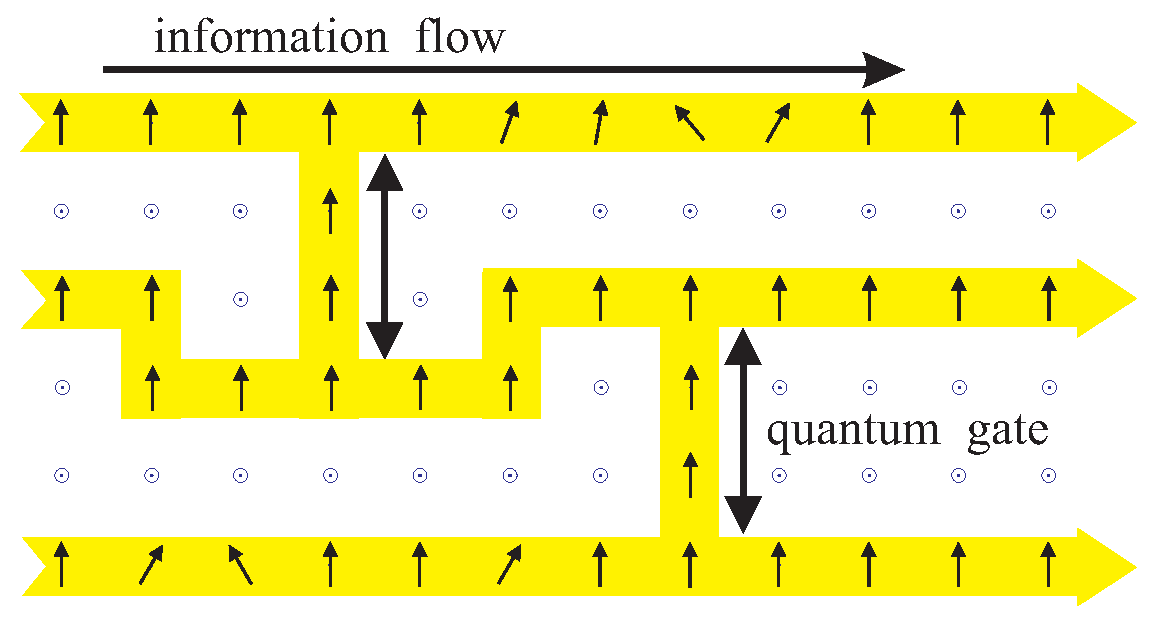
\includegraphics[
    width=0.75\textwidth
    ]{fig/flow.eps}
  \caption{Simulation of a quantum circuit with a one-way computer. Horizontal direction simulates the circuit's time evolution and vertical direction represents the qubit register. \(\odot\) vertices denote a measurement along \(\sigma_z\), a vertical arrow denotes a measurement along \(\sigma_x\) and a tilted arrow denotes a measurement along the \(xy\) plane. The image by Raussendorf et. al.\cite{russendorf2003}} \label{fig:flow}
\end{figure}

After introducing a general framework for simulating quantum circuits, we introduce two additional measurement patterns. The first one among these is a measurement by \(\sigma_z\). This measurement effectively deletes a vertex from the cluster without affecting the program logic. A 2 qubit cluster state with an input \(\ket{\psi} = a\ket0+b\ket1\) has the following quantum state.
\begin{align}
  \ket{G} &= CZ\ket\psi\ket+\\
  &= \frac{1}{\sqrt2}(a\ket{00} + a\ket{01} + b\ket{10} - b\ket{11})
\end{align}
Measuring the second qubit will yield \(a\ket0+b\ket1\) if the outcome is 0, and it will yield \(a\ket0-b\ket1\) if otherwise. So a measurement on \(\sigma_z\) removes the qubit with a side effect operator \(\sigma_z^s\).

The last measurement pattern is the \(\sigma_x\) measurement, which propagates the information in a linear cluster to the next vertex. The by-product operators are cyclic, with a period of four propagations.
\begin{equation}
  U_\Sigma =  \sigma_x^{s_1} \sigma_z^{s_2}
\end{equation}